\subsection{Clustering}

\subsubsection{Clustering evaluation metrics}

To evaluate clustering, the metrics used are the BCubed~\cite{bcubed} family (called sometimes $B^3$, in this report).
BCubed has shown to satisfy 4 following importants constraints when evaluating clusterings : \textit{Cluster Homogeneity} (different categories should be in the different clusters), \textit{Cluster Completness} (same categories should belong to the same cluster) and the \textit{Rag Bag constraint} (noisy/miscellaneous categories should be in the same cluster and not in 'healthy' clusters) and the \textit{Cluster size vs quantity constraints} (favorise large cluster)~\cite{bcubed}.
These metrics are used in the clustering task at PAN @ CLEF~\cite{pan16}.

\begin{definition}[Correctness~\cite{bcubed}]
  The $BCubed$ metric family is based on the the following \textit{Correctness} principle.
  Let L(e) and C(e) be the category and the cluster of an element e.
  The Correctness is following the biconditional condition on the category and cluster equality (biconditional: $A \Longleftrightarrow B \equiv (A \land B) \lor (\neg A \land \neg B)$).
  \begin{gather*}
    Correctness(e, e') = \\
    \begin{cases}
      1, & if (L(e) = L(e')) \Longleftrightarrow (C(e) = C(e'))\\
      0, & otherwise
    \end{cases}
  \end{gather*}
  In other terms, the correctness has a value of one (100\% correct) if the two elements are in the both in the same cluster and has the same category OR both in a different cluster and a different category.
\end{definition}

\begin{definition}[$BCubed$ Precision~\cite{bcubed}]
  The $BCubed$ Precision correspond to the average of correctness for all elements on the average of all element such that \textbf{their clusters are the same}.
  \begin{equation}
    B^3_{precision} = \text{Avg}_{e}[\text{Avg}_{e' C(e)=C(e')}[Correctness(e, e')]]
  \end{equation}
\end{definition}

\begin{definition}[$BCubed$ Recall~\cite{bcubed}]
  The $BCubed$ Recall correspond to the average of correctness for all elements on the average of all element such that \textbf{their categories are the same}.
  \begin{equation}
    B^3_{recall} = \text{Avg}_{e}[\text{Avg}_{e' L(e)=L(e')}[Correctness(e, e')]]
  \end{equation}
\end{definition}

\begin{definition}[$BCubed F_1$ Score~\cite{bcubed}]
  $BCubed F_1$ Score uses the harmonic mean between the $B^3_{precision}$ and $B^3_{recall}$.
  \begin{equation}
    B^3_{F_1} =
    2 \cdot \frac{B^3_{precision} \cdot B^3_{recall}}
    {B^3_{precision} + B^3_{recall}}
  \end{equation}
  The $F_\beta$ measures, not shown here, provide a parametric way to represent with a single value the two counterbalancing measures in this case, the $B^3_{F_1}$ is computed using the $F$ measures with $\beta = 1$ and the $B^3_{precision}$ and $B^3_{recall}$ scores.
\end{definition}

An additional metric introduced and used in this study is the Cluster difference.

\begin{definition}[Cluster difference]
  This metric aim to evaluate if the clustering found the right number of cluster.
  The cluster difference is the number cluster found $p$ minus the actual number of cluster $k$.
  \begin{equation}
    Cluster_{diff} = p - k
  \end{equation}
  A positive value indicate an overestimation of the real number of cluster, a negative value indicate the underestimation.
  Zero indicate that the right number of cluster was found.
  This value can be normalized by the number of documents N, which correspond to the difference of the r ratios.
  As stated in the PAN16 evaluation campaign paper, estimating correctly the r ratio tends to indicate a good clustering~\cite{pan16}.
  \begin{equation}
    r_{diff} = \frac{p}{N} - \frac{k}{N} = \frac{p - k}{N}
  \end{equation}
\end{definition}

\subsubsection{Hierarchical clustering parameters}

As explained in Section~\ref{sec:authors_clustering}, the hierarchical clustering decide clusters based on bottom-up approach and have two main parameters, the stopping criterion and the linkage criterion.
In this experiment, the goal is two find the best criterion our dataset for both stopping procedures.
For the stopping procedure based on the number of cluster, used in the unsupervised clustering approach, the agglomerative clustering is stopped at the right number of cluster, this depends on the corpus.
Then the $B^3_{F_1}$ score is computed for every corpus and linkage criterion.
But for the distance threshold stop procedure, the right distance threshold is not known, so the idea is to stop the algorithm at each merging step, evaluate the solution using the $B^3_{F_1}$ score and only retain the best score for each dataset and criterion.
Since the libraby used does not provide a simple way to stop at each merge, a trick was used to avoid re-implementing or modifing the algorithm, which concist to increase the distance threshold by a small value until the number of clusters found is the greater then number of authors.
The $B^3_{F_1}$ score retained is the maximal reached during every steps.
The step should be small enough to ensure that the algorithm is stopped at each merging at least.
This method is high inefficiant and is only used to get the results needed for the choice in criterion.
If the step is small enough, and not merging are missed, the value obtained is guaranteed to be the optimal clustering for this rank list.

The results for both stopping procedure are presented in Table~\ref{tab:clustering_linkages}.
On every corpus the average linkage criterion $B^3_{F_1}$ score is better or equal to the single and complete linkage score which results in  average to a better linkage criterion.
The average linkage criterion is used for every subsequent experiments.

\begin{table}
  \centering
  \caption{$B^3_{F_1}$ over linkage criterion for every corpus}
  \label{tab:clustering_linkages}

  \subcaption{Using the number of cluster as stopping procedure}
  \label{tab:clustering_linkages_stop_clusters}
  \begin{tabular}{l c c c}
    \toprule
           & \multicolumn{3}{c}{Linkage criterion} \\
    Corpus & Single & Complete & Average \\
    \midrule
    Oxquarry  & 0.81 & 0.81 & 0.82 \\
    Brunet    & 0.81 & 0.79 & 0.81 \\
    St-Jean A & 0.85 & 0.85 & 0.85 \\
    St-Jean B & 0.96 & 0.97 & 0.97 \\
    St-Jean   & 0.79 & 0.87 & 0.88 \\
    \midrule
    Mean      & 0.84 & 0.86 & 0.87 \\
    \bottomrule
  \end{tabular}

  \subcaption{Using the distance threshold as stopping procedure}
  \label{tab:clustering_linkages_stop_distance_threshold}
  \begin{tabular}{l c c c}
    \toprule
           & \multicolumn{3}{c}{Linkage criterion} \\
    Corpus & Single & Complete & Average \\
    \midrule
    Oxquarry  & 0.89 & 0.87 & 0.89 \\
    Brunet    & 0.84 & 0.85 & 0.86 \\
    St-Jean A & 0.86 & 0.87 & 0.87 \\
    St-Jean B & 0.98 & 0.97 & 0.99 \\
    St-Jean   & 0.87 & 0.90 & 0.89 \\
    \midrule
    Mean      & 0.89 & 0.89 & 0.90 \\
    \bottomrule
  \end{tabular}
\end{table}

\subsubsection{Unsupervised clustering evaluation}

For this experiment, the goal is to test the unsupervised cut method based on the IPS (Iterative positive silhouette) Procedure on the literature dataset.
When applying the procedure, the number of clusters start at 2, each iteration the silhouette score is computed if it reaches a negative value the procedure stop otherwise the number of cluster is increased and the process is repeated.

The rank list used for this experiment is the one generated using Z-score fusion with retained text representation (9 for St-Jean and 7 for Brunet and Oxquarry), see Section~\ref{sec:annex_retained_text_representation} in annex.

When running the IPS procedure on the dataset, on Figures~\ref{fig:unsupervised_clustering} the silhouette score is indicated as each step and compared to the three BCubed metrics.
For the sake of the experiment, the agglomerative clustering is also run up to a number of cluster equal to the number of documents (singleton clusters).
The detailed score on the unsupervised clustering is presented in Table~\ref{tab:unsupervised_clustering_0}.

Since the rank list used for the clustering is not perfect (every true links at the top), there is no number of cluster with a BCubed $F_1$ score of 1.0.
The estimated number of cluster is on every dataset overestimated, since the average r-ratio difference is positive $0.21$ and the $B^3_{precision}$ is larger than the $B^3_{recall}$, which means that the median neareast-cluster distance is greater than the median intra-cluster distance even when dealing with the right number of clusters.
This can be due to the fact that the rank list used for the clustering is not perfect (AP $\neq 1$).

To mitigate this problem, an easy solution would be to the stop the procedure at for example : $0.1$ instead of $0$.
When running the IPS with a stop at $0.1$ on the dataset, the obtained results are presented in Table~\ref{tab:unsupervised_clustering_01}.
The average r-ratio difference drop to $0.13$, which result in a 38\% improvement when stopping the procedure at $0.1$ instead of $0$, this tweaking seem to improve the results, especially for the St-Jean A corpus, which have an relative $B^3_{F_1}$ increase of +24\%.
No solid founding are used for tweaking this parameter.

To further improve the results, instead of iterating on the number of clusters as proposed in the original paper~\cite{automated_unsupervised}, iterating over the distance threshold can improve the results, but increase the complexity.

\begin{table}
  \centering
  \caption{Unsupervised clustering evaluation on the datasets}
  \label{tab:unsupervised_clustering}

  \subcaption{IPS Standard Procedure (stop at 0.0)}
  \label{tab:unsupervised_clustering_0}
  \begin{tabular}{l c c c c}
    \toprule
    &
    $B^3_{F_1}$ &
    $B^3_{precision}$  &
    $B^3_{recall}$  &
    $r_{diff}$ \\
    \midrule
    Oxquarry         & 0.73 & 1.00 & 0.58 & 0.23\\
    Brunet           & 0.82 & 0.94 & 0.73 & 0.11\\
    St-Jean A        & 0.64 & 1.00 & 0.47 & 0.22\\
    St-Jean B        & 0.74 & 1.00 & 0.59 & 0.26\\
    \textbf{Average} &
    \textbf{0.73} &
    \textbf{0.99} &
    \textbf{0.59} &
    \textbf{0.21} \\
    \bottomrule
  \end{tabular}

  \subcaption{IPS Procedure with stop at 0.1}
  \label{tab:unsupervised_clustering_01}
  \begin{tabular}{l c c c c}
    \toprule
    &
    $B^3_{F_1}$ &
    $B^3_{precision}$  &
    $B^3_{recall}$  &
    $r_{diff}$ \\
    \midrule
    Oxquarry         & 0.74 & 1.00 & 0.59 & 0.21\\
    Brunet           & 0.82 & 0.82 & 0.82 & 0.05\\
    St-Jean A        & 0.84 & 0.89 & 0.79 & 0.03\\
    St-Jean B        & 0.77 & 1.00 & 0.62 & 0.21\\
    \textbf{Average} &
    \textbf{0.79} &
    \textbf{0.93} &
    \textbf{0.71} &
    \textbf{0.13} \\
    \bottomrule
  \end{tabular}
\end{table}

\begin{figure}
  \caption{Unsupervised clustering example on Brunet and St-Jean B}
  \label{fig:unsupervised_clustering}

  \subcaption{Brunet}
  \label{fig:unsupervised_clustering_brunet}
  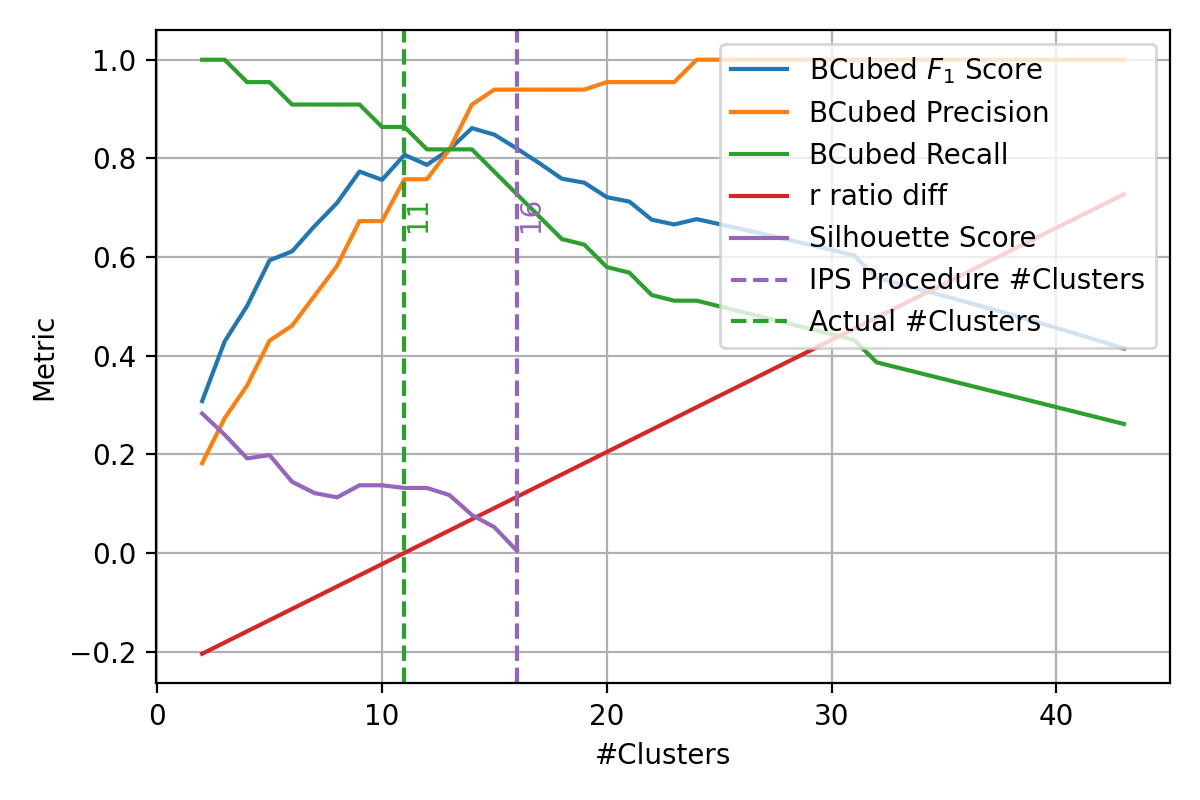
\includegraphics[width=\linewidth]{img/unsupervised_clustering_brunet.png}

  \subcaption{St-Jean B}
  \label{fig:unsupervised_clustering_st_jean_B}
  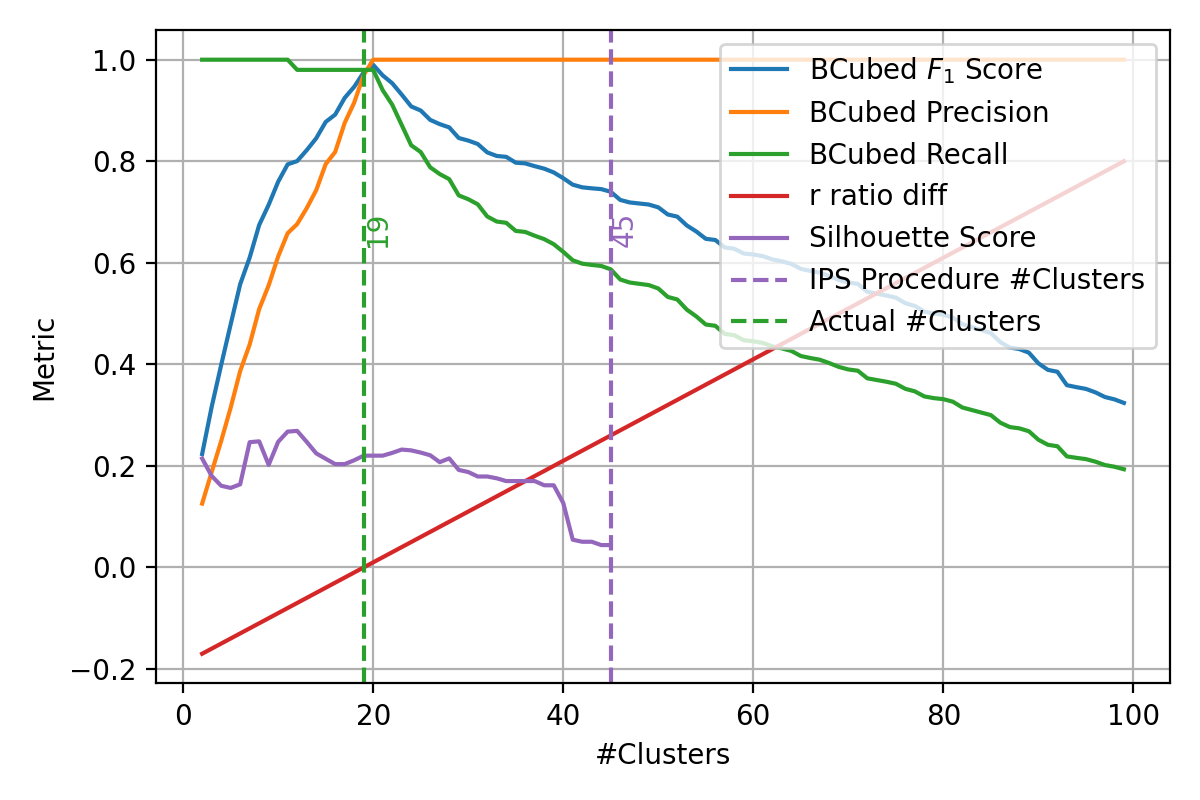
\includegraphics[width=\linewidth]{img/unsupervised_clustering_st_jean_B.png}
\end{figure}


\subsubsection{Semi-supervised clustering evaluation}

To evaluate the semi-supervised clustering approach, every corpus were used.
First a rank list for each corpus is computed using a z-score fusion using the retained rank list, see Section~\ref{sec:annex_retained_text_representation} in annex.
For each rank list, the distance threshold is computed, using the two beta approach, this correspond to the training phase.
Then for every distance threshold and rank list pair, the clustering is evaluated using the $B^3$ family and the $r_{diff}$.

The distance thresholds found for the z-score fusion rank lists for each corpus are in Table~\ref{tab:semi_supervised_clustering_thresholds}
The complete evaluation using Oxquarry, Brunet, St-Jean A and B, is presented in Table~\ref{tab:semi_supervised_clustering_train_test}.
The average values obtained for each metrics is presented in Table~\ref{tab:semi_supervised_clustering_average}.

The following conclusions can be drawn with these results:
\begin{itemize}
  \item
  A rather wide range of distance threshold is found depending on the corpus. They are in the interval $\left[-0.42, -0.96\right]$ which correspond to 14\% of the interval containing every z-scores for these datasets ($\left[-4.79, 2.63\right]$).
  \item
  The average r-ratio is positive, which indicate that this method tends to overestimate the number of clusters, but is really close to find the right number of clusters.
  \item
  The better the average precision of the rank list used, the better the $B^3_{F_1}$ score seem to be, when using this method, with the exception of the Oxquarry corpus which have better average precision then Brunet but a lower $B^3_{F_1}$ score in average when testing with these corpora.
  \item
  The distance threshold use only have a slight impact when comparing the average $B^3_{F_1}$ score across the corpus.
  The St-Jean A corpus give the best $B^3_{F_1}$ and regarding the number of clusters Oxquarry seem to be the best corpus for the training.
\end{itemize}

The semi-supervised cut method tends to produce better results in average than the unsupervised proposed method.
An increase of +8\% in $B^3_{F_1}$ can be obtained when using the supervised clustering model proposed over the unsupervised tweaked clustering model (IPS stop procedure at 0.1) and +15\% over the IPS stop procedure at 0.

\begin{table}
  \centering
  \caption{Distance threshold found with the two beta distribution on every corpora when using the z-score fusion of the retained rank lists}
  \label{tab:semi_supervised_clustering_thresholds}

  \begin{tabular}{l r}
    \toprule
    Corpus & Threshold \\
    \midrule
    Oxquarry & -0.42 \\
    Brunet & -0.62 \\
    St-Jean A & -0.76 \\
    St-Jean B & -0.96 \\
    \bottomrule
  \end{tabular}
\end{table}

\begin{table*}
  \centering
  \caption{Semi-supervised clustering evaluation}
  \label{tab:semi_supervised_clustering}

  \subcaption{Every possible distance threshold (DT) and retained z-score rank list pairs. Metrics in order : $B^{3}_{F_1}$ / $B^{3}_{precision}$ / $B^{3}_{recall}$ / $r_{diff}$}
  \label{tab:semi_supervised_clustering_train_test}
  \begin{tabular}{l l| c c c c}
    \toprule
    \multicolumn{2}{c}{\multirow{2}{*}{}} & \multicolumn{4}{c}{Testing} \\
    \multicolumn{2}{c}{} & Oxquarry & Brunet & St-Jean A & St-Jean B \\
    \midrule
    \parbox[t]{2mm}{\multirow{4}{*}{\rotatebox[origin=c]{90}{DT}}}
    & Oxquarry
    & 0.82/1.00/0.70/0.08
    & 0.81/0.85/0.77/0.07
    & 0.86/0.84/0.87/-0.02
    & 0.91/0.86/0.98/-0.03
    \\
    & Brunet
    & 0.82/1.00/0.70/0.08
    & 0.81/0.85/0.77/0.07
    & 0.87/0.86/0.87/-0.01
    & 0.92/0.88/0.98/-0.02
    \\
    & St-Jean A
    & 0.82/1.00/0.70/0.08
    & 0.85/0.94/0.77/0.09
    & 0.87/0.86/0.87/-0.01
    & 0.97/0.97/0.98/0.00
    \\
    & St-Jean B
    & 0.80/1.00/0.67/0.10
    & 0.84/1.00/0.73/0.14
    & 0.84/0.93/0.77/0.04
    & 0.90/0.97/0.83/0.04
    \\
    \bottomrule
  \end{tabular}

  \subcaption{Metrics averages}
  \label{tab:semi_supervised_clustering_average}
  \begin{tabular}{l c c c c}
    \toprule
    & $B^{3}_{F_1}$
    & $B^{3}_{precision}$
    & $B^{3}_{recall}$
    & $r_{diff}$ \\
    \midrule
    Testing on Oxquarry               & 0.82 & 1.00 & 0.69 &  0.08 \\
    Testing on Brunet                 & 0.83 & 0.91 & 0.76 &  0.09 \\
    Testing on St-Jean A              & 0.86 & 0.88 & 0.85 &  0.00 \\
    Testing on St-Jean B              & 0.93 & 0.92 & 0.94 & -0.00 \\
    Distance threshold from Oxquarry  & 0.85 & 0.89 & 0.83 & 0.02 \\
    Distance threshold from Brunet    & 0.86 & 0.90 & 0.83 & 0.03 \\
    Distance threshold from St-Jean A & 0.88 & 0.94 & 0.83 & 0.04 \\
    Distance threshold from St-Jean B & 0.85 & 0.98 & 0.75 & 0.08 \\
    \textbf{Global average} & \textbf{0.86} & \textbf{0.93} & \textbf{0.81} & \textbf{0.04} \\
    \bottomrule
  \end{tabular}
\end{table*}

\subsubsection{Supervised clustering evaluation}

To evaluate the supervised clustering approach, every dataset were used.
First a rank list for each dataset is computed using a z-score fusion using the retained rank list, see Section~\ref{sec:annex_retained_text_representation} in annex.
Then every pair of rank list is used to create a training/testing evaluation.
In other words, a model to create cuts is trained on every dataset and tested on all the datasets.

The model does not depend on the rank list size since only relative magnitudes are used.
The BCubed $F_1$ metrics and the r ratio difference are computed during this experiment and are in presented in Table~\ref{tab:supervised_clustering_train_test}, for every pairs of dataset.
The average values obtained for each metrics is presented in Table~\ref{tab:supervised_clustering_average}.

Two conclusion can be drawn with these results:
\begin{itemize}
  \item
  When testing the cut model, having a rank list of good quality tends to produce better clustering, no matter the quality of the rank list used for the training.
  When testing the clustering model on St-Jean B (the corpus with the best rank list obtained, 0.96 AP), it obtains in average the best $B^3_{F_1}$ 0.93 for any training model.
  The least performing rank list also have the least accurate results during the clustering task, Brunet with 0.76 AP have an average clustering $B^3_{F_1}$ of 0.80.
  \item
  Using the best rank list for training the cut model does not always give the best results.
  An example to illustrate this observation, the St-Jean B dataset have the best rank list with an average precision of 0.96, but the best rank list for training the clustering model is Oxquarry with an average $r_{diff}$ of 0.02 and an average $B^3_{F_1}$ of 0.87.
  In the other hand, St-Jean B have an average $r_{diff}$ of 0.09 and an average $B^3_{F_1}$ of 0.83.
  The Oxquarry rank list seem to be the best dataset to train the model to perform the cut and Brunet the least effective.
\end{itemize}

The conclusion to the two previous points is that having a good rank list is more important for testing than training.
No clear rank lists property was found which makes some of them better to train the model.
The supervised cut method tends to produce better results in average than the unsupervised proposed method.
An increase of +8\% in $B^3_{F_1}$ can be obtained when using the supervised clustering model proposed over the unsupervised tweaked clustering model (IPS stop procedure at 0.1) and +14\% over the IPS stop procedure at 0.

\begin{table*}
  \centering
  \caption{Supervised clustering evaluation}
  \label{tab:supervised_clustering}

  \subcaption{Every possible threshold and dataset pairs. Metrics in order : $B^{3}_{F_1}$ / $B^{3}_{precision}$ / $B^{3}_{recall}$ / $r_{diff}$}
  \label{tab:supervised_clustering_train_test}
  \begin{tabular}{l l| c c c c}
    \toprule
    \multicolumn{2}{c}{\multirow{2}{*}{}} & \multicolumn{4}{c}{Testing} \\
    \multicolumn{2}{c}{} & Oxquarry & Brunet & St-Jean A & St-Jean B \\
    \midrule
    \parbox[t]{2mm}{\multirow{4}{*}{\rotatebox[origin=c]{90}{Training}}}
    & Oxquarry
    & 0.82/1.00/0.70/0.08
    & 0.86/0.91/0.82/0.07
    & 0.88/0.84/0.93/-0.03
    & 0.92/0.88/0.98/-0.02
    \\
    & Brunet
    & 0.80/1.00/0.67/0.10
    & 0.75/0.94/0.62/0.18
    & 0.81/0.98/0.69/0.09
    & 0.91/1.00/0.83/0.05
    \\
    & St-Jean A
    & 0.80/1.00/0.67/0.10
    & 0.82/0.94/0.73/0.11
    & 0.87/0.93/0.81/0.03
    & 0.97/1.00/0.94/0.02
    \\
    & St-Jean B
    & 0.80/1.00/0.67/0.10
    & 0.76/0.94/0.64/0.16
    & 0.82/0.96/0.72/0.07
    & 0.93/1.00/0.84/0.04
    \\
    \bottomrule
  \end{tabular}

  \subcaption{Metrics averages}
  \label{tab:supervised_clustering_average}
  \begin{tabular}{l c c c c}
    \toprule
    & $B^{3}_{F_1}$
    & $B^{3}_{precision}$
    & $B^{3}_{recall}$
    & $r_{diff}$ \\
    \midrule
    Testing on Oxquarry     & 0.81 & 1.00 & 0.68 & 0.09 \\
    Testing on Brunet       & 0.80 & 0.93 & 0.70 & 0.13 \\
    Testing on St-Jean A    & 0.85 & 0.93 & 0.79 & 0.04 \\
    Testing on St-Jean B    & 0.93 & 0.97 & 0.91 & 0.02 \\
    Training on Oxquarry    & 0.87 & 0.91 & 0.86 & 0.02 \\
    Training on Brunet      & 0.82 & 0.98 & 0.71 & 0.10 \\
    Training on St-Jean A   & 0.86 & 0.97 & 0.79 & 0.06 \\
    Training on St-Jean B   & 0.83 & 0.97 & 0.73 & 0.09 \\
    \textbf{Global average} & \textbf{0.85} & \textbf{0.96} & \textbf{0.77} & \textbf{0.07} \\
    \bottomrule
  \end{tabular}
\end{table*}
